\section{The energy balance law}\label{sec:19.5}

A silicon recoil of \SI{1}{keV} makes about 34 electron--hole pairs, at the measured ionization yield $Y_q = 0.127$ (\cref{sec:19.2}) and $\varepsilon_{\mathrm{eh}} = \SI{3.75}{eV}$, and their gap energy is \SI{40}{eV}. The rest of the deposit is phonons and, if the recoil displaced atoms, stored energy. A millisecond later the phonons have been absorbed at the surfaces of the crystal, most pairs have returned their gap energy as phonons and a few are caught on traps, while the defects still hold their energy. A phonon sensor reads the share that reached it within its readout window, and a calibration made with electron recoils converts that reading into an energy. The conversion is correct when electron and nuclear recoils of the same energy deliver the same share. To see when that holds, we write one law that tracks every share at every time. Applied to the silicon calibration of the CDMS~II detectors, the law shows that the measured ratio fixes a combination of stored energy, phonon collection and the pair energy of the reconstruction, which a second bias can separate.

\subsection{Reservoirs of the deposit}\label{sec:19.5-law}

At the partition time $t_{\mathrm{pr}}$ the deposit $\omega$ is split as in \cref{eq:19.1-heat}: $N_{\mathrm{eh}}\Eg$ in pairs, $E_{\mathrm{st}}$ in defects and $E_{\mathrm{heat}}$ in phonons. After $t_{\mathrm{pr}}$ the energy keeps moving. Pairs bind into excitons, recombine, are captured on impurities or drift to the electrodes, defects release their energy (\cref{sec:19.6}), and the phonons leave the crystal through its surfaces. Five reservoirs hold the energy at any time $t$. Write $E_{\mathrm{dep}} \equiv \omega$ for the deposit when it is divided among them.

The carriers hold $E_{\mathrm{pairs}}(t)$. Each energy is counted from the Fermi level $\mu_F$ of the electrodes, as in \cref{sec:18.5}: a free electron holds $E_c - \mu_F$, a free hole $\mu_F - E_v$, an exciton $\Eg - E_x^b$, an electron trapped on a level $E_j$ holds $E_j - \mu_F$ and a trapped hole $\mu_F - E_j$. To these we add the electrostatic energy of the charge left in the crystal, the Coulomb energy of separated carriers, their images in the electrodes and any space charge. The phonons hold $E_{\mathrm{phon}}(t)$, the vibrational energy above the thermal bath; its value at $t_{\mathrm{pr}}$ is the prompt phonon energy $E_{\mathrm{prompt}} \equiv E_{\mathrm{phon}}(t_{\mathrm{pr}})$. The defects hold the stored energy $E_{\mathrm{st}}(t)$, a difference of minima of $E^{\mathrm{ad}}$ as in \cref{eq:19.1-partition}. The escaped energy $E_{\mathrm{esc}}(t)$ is carried out of the crystal by quanta that no surface absorbs, in practice luminescence photons. Last, $E_{\mathrm{sens}}(t)$ is the energy absorbed at the surfaces: by the sensor films, of which a part becomes signal, and by holders and uninstrumented faces. A bias source at fixed voltage adds the work $W_{\mathrm{bias}}(t)$ it has done on the drifting charge.
\begin{keyresult}[Energy balance law]
At every time $t$ after the deposit, and for every event,
\begin{equation}
  E_{\mathrm{dep}} + W_{\mathrm{bias}}(t) =
  \underbrace{E_{\mathrm{pairs}}(t)}_{\text{carriers}} +
  \underbrace{E_{\mathrm{phon}}(t)}_{\text{phonons}} +
  \underbrace{E_{\mathrm{st}}(t)}_{\text{defects}} +
  \underbrace{E_{\mathrm{esc}}(t)}_{\text{escaped}} +
  \underbrace{E_{\mathrm{sens}}(t)}_{\text{absorbed}} ,
  \label{eq:19.5-balance}
\end{equation}
with carrier energies counted from the Fermi level of the electrodes, the stored energy configurational, and the change of zero-point energy of the occupied defect basins inside $E_{\mathrm{phon}}$.
\end{keyresult}
\noindent \Cref{app:D.45} proves \cref{eq:19.5-balance} from the conservation of the total energy of crystal, sensors, radiation and bias source. Apart from the work of the source, the total energy is conserved. Between collisions it equals the sum of the reservoir energies, since the interactions of excited carriers with each other are either long-range Coulomb energy, which $E_{\mathrm{pairs}}$ contains, or short-range energy that acts during a collision alone. Every process after $t_{\mathrm{pr}}$ is a short-range transition that conserves energy, or a drift whose energy the bias work and the electrostatic energy account for. The law holds for each realization of the random sequence of captures, hops and absorptions, and hence also in the mean. Its content is the completeness of the reservoir list. At $t_{\mathrm{pr}}$ and zero field, with no capture, it is the partition: $E_{\mathrm{pairs}} = N_{\mathrm{eh}}\Eg$, $E_{\mathrm{prompt}} = E_{\mathrm{heat}}$, $E_{\mathrm{esc}} = E_{\mathrm{sens}} = 0$, and \cref{eq:19.5-balance} is \cref{eq:19.1-heat}.

The Fermi level of the electrodes is the one reference for the carrier energies that keeps the law closed. A carrier that reaches an electrode gives up its energy relative to the Fermi level of that electrode, as phonons at the contact; the CDMS~II analysis names these the recombination phonons~\cite[Sect.~2]{agnese2018nuclear}. Counted from another level $\mu$, the carriers still in the crystal hold an energy whose derivative with respect to $\mu$ is the number of holes minus the number of electrons among them. That number is zero as long as every carrier still has its partner. Once one carrier of a pair has been collected and the other has not, energies counted from $\mu \ne \mu_F$ change with the arbitrary $\mu$, and the balance no longer closes. A hole left behind when its electron is collected thus stores $\mu_F - E_v$, plus its image energy, and not half the gap.

The stored energy enters once. The displacement threshold appears nowhere in \cref{eq:19.5-balance}. The stored energy decreases through releases alone, each of which moves its energy to $E_{\mathrm{phon}}$, or to $E_{\mathrm{esc}}$ if a photon carries it away. A calibration that subtracts an energy per displaced atom from the heat and also counts the later release as heat counts the same energy twice.

The zero-point energy of the occupied basins sits inside $E_{\mathrm{phon}}$. A defect softens or stiffens the modes of its neighbors and so changes the zero-point energy of the crystal by an amount $\Delta E_{\mathrm{zp}}(t)$, which \cref{sec:19.1-partition} placed in the lattice share. It is the energy of the vibrational ground state, and no sensor can absorb it. Its size follows from the zero-point energy per silicon atom, $3\langle\omega\rangle/2 = \SI{61}{meV}$, half of it the potential energy of \cref{sec:19.1-md}. A point defect that shifts the frequencies of its four neighbors by some tens of percent changes $\Delta E_{\mathrm{zp}}$ by about \SI{0.07}{eV}, an estimate, against the several eV a Frenkel pair stores. The sign is not fixed: softened modes make $\Delta E_{\mathrm{zp}}$ negative, stiffened ones positive. A defect that hops from basin $i$ to basin $j$ releases into the phonons the configurational difference plus the change of zero-point energy between the two basins. Summed along any release path, the zero-point terms telescope like the configurational ones, so the sum rule of \cref{sec:19.6} holds for both separately. A sensor can draw on $E_{\mathrm{phon}} - \Delta E_{\mathrm{zp}}$ alone.

The Luke effect enters the balance through the bias work. A carrier drifting at constant velocity in the field of a biased detector gains from the field the energy $e\mathcal{E}$ per unit path and gives it to phonons as fast as it gains it: the Neganov--Trofimov--Luke effect of \cref{eq:1.5-luke}, whose emission spectrum \cref{sec:20.1} treats. Between two planar electrodes at fixed potentials, a carrier that crosses a fraction $s$ of the gap induces the charge $es$ on the electrodes, and the source does the work $eV_{\mathrm{bias}}s$ on it (Ramo's theorem, \cref{app:D.45}). The total work is
\begin{equation}
  W_{\mathrm{bias}} = eV_{\mathrm{bias}}N_{\mathrm{ind}} ,
  \label{eq:19.5-Wbias}
\end{equation}
where $N_{\mathrm{ind}}$ is the induced charge in units of $e$, equal to the number of pairs if all are collected and smaller if carriers are trapped on the way. Of this work, $W_{\mathrm{bias}}$ minus the change of the electrostatic energy goes to phonons; for pairs born neutral and fully collected the electrostatic term vanishes at the end. For an electron recoil, whose pair number is $\omega/\varepsilon_{\mathrm{eh}}$, the ratio of the Luke phonon energy to the deposit is the Luke gain
\begin{equation*}
  g_{\mathrm{Luke}} = \frac{eV_{\mathrm{bias}}}{\varepsilon_{\mathrm{eh}}} ,
\end{equation*}
1.07 at \SI{4}{V} and 26.7 at \SI{100}{V} in silicon. Carriers already drift during the cascade, before $t_{\mathrm{pr}}$, over the short distance they travel in that time; that work is part of the same $W_{\mathrm{bias}}$ and of the same Luke phonons.

\Cref{fig:19-shares} follows the five reservoirs of a \SI{1}{keV} silicon recoil at zero field. The pair kinetics are those of \cref{fig:18-end}: the gap energy is released within microseconds, except for the \SI{5}{\percent} of pairs that the illustrative rates trap and the \SI{0.9}{\percent} that leave as light. The phonons are absorbed with a single time constant of \SI{58}{\micro s}, the fall time of the pulse of a \SI{10.6}{g} silicon phonon detector~\cite[p.~2]{alkhatib2021light}. After a millisecond the surfaces have absorbed \SI{943}{eV}, the traps keep \SI{2.0}{eV} and the defects their full \SI{55}{eV}. For a stated detector the evolution of the reservoirs is a transport calculation: the charge kinetics, Luke emission and collection at the surfaces of \cref{app:E.25}, started from the partition tables of \cref{app:E.23}.

\begin{figure}[tbp]
  \centering
  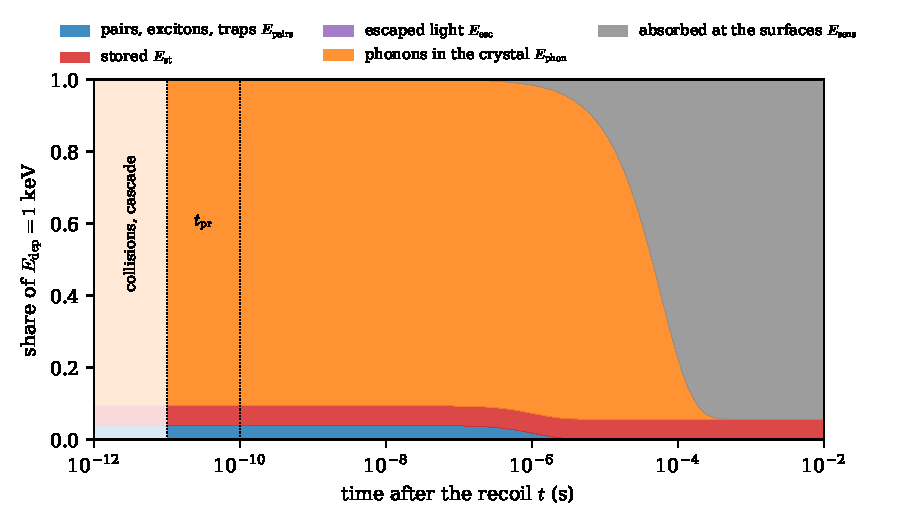
\includegraphics[width=\linewidth]{figures/ch19/fig19_4.pdf}
  \caption{Shares of the balance law \cref{eq:19.5-balance} for a \SI{1}{keV} silicon recoil at zero field, against the time after the recoil, as fractions of $E_{\mathrm{dep}}$. At the partition time $t_{\mathrm{pr}}$ (dotted lines, 10 to \SI{100}{ps}): $N_{\mathrm{eh}} = 33.9$ pairs from the measured yield $Y_q = 0.127$ at \SI{0.89}{keV}~\cite[Table~II]{albakry2023first} with $\varepsilon_{\mathrm{eh}} = \SI{3.75}{eV}$, holding $N_{\mathrm{eh}}\Eg = \SI{39.6}{eV}$ with $\Eg = \SI{1.17}{eV}$; stored energy set to \SI{55}{eV}, the silicon bound of \cref{tab:19-bounds}, for display, and kept frozen; phonons \SI{905}{eV}. Pair kinetics: the illustrative rates of \cref{fig:18-end} (one free pair per pair, \SI{5}{\percent} trapped, luminescent fraction 0.1 of free-exciton decay, bound-exciton Auger decay \SI{250}{ns}); trapped carriers stay in $E_{\mathrm{pairs}}$. Phonons absorbed at the surfaces with one exponential time constant, \SI{58}{\micro s}, the pulse fall time of a silicon phonon detector~\cite[p.~2]{alkhatib2021light}, a modeling choice. Shares at \SI{10}{ms}: absorbed 0.943, stored 0.055, trapped 0.002, escaped $3\times10^{-4}$. The collisions and the cascade before $t_{\mathrm{pr}}$ are not resolved.}
  \label{fig:19-shares}
\end{figure}

\subsection{Heat quenching}\label{sec:19.5-heat}

Without bias the phonon sensors measure the heat. Their readout integrates the energy absorbed during a window $t_{\mathrm{win}}$, from microseconds to a second depending on the sensor, and the phonons still in the crystal at the end of the window are absorbed with the same pulse shape whatever made them. Energy that has not become available phonons by $t_{\mathrm{win}}$ is missing from the signal for good. It is the sum of the energy still held by carriers, the energy still stored, the escaped energy and the zero-point change,
\begin{equation*}
  E_{\mathrm{miss}}(t_{\mathrm{win}}) = E_{\mathrm{pairs}}(t_{\mathrm{win}}) + E_{\mathrm{st}}(t_{\mathrm{win}}) + E_{\mathrm{esc}}(t_{\mathrm{win}}) + \Delta E_{\mathrm{zp}}(t_{\mathrm{win}}) .
\end{equation*}
The sensors turn a fraction $\epsilon_{\mathrm{abs}}$ of the available phonon energy into signal, $\epsilon_{\mathrm{abs}}(E_{\mathrm{dep}} - E_{\mathrm{miss}})$; the rest goes into $E_{\mathrm{sens}}$ as loss on uninstrumented faces and in the films. This fraction is often well below one, but it is the same for every event of a given kind of recoil at a given place. Let $\epsilon^{\mathrm{NR}}_{\mathrm{prim}}$ and $\epsilon^{\mathrm{ER}}_{\mathrm{prim}}$ be its values for the primary phonons of nuclear and electron recoils, the sole phonons at zero field, and define the collection offset $\delta_{\mathrm{coll}} \equiv 1 - \epsilon^{\mathrm{NR}}_{\mathrm{prim}}/\epsilon^{\mathrm{ER}}_{\mathrm{prim}}$. The heat quenching is the ratio of the heat signals of a nuclear and an electron recoil of the same energy,
\begin{equation}
  Y_{\mathrm{ph}}(0) = (1 - \delta_{\mathrm{coll}})\,\frac{1 - d_{\mathrm{NR}}}{1 - d_{\mathrm{ER}}} , \qquad
  d_{\mathrm{NR},\mathrm{ER}} \equiv \frac{E^{\mathrm{NR},\mathrm{ER}}_{\mathrm{miss}}(t_{\mathrm{win}})}{\omega} ,
  \label{eq:19.5-heatq}
\end{equation}
the zero-field value of the phonon-yield ratio $Y_{\mathrm{ph}}$ defined in \cref{sec:19.5-yield}. The absolute efficiency has dropped out, and with it the large losses at the surfaces; what remains is the difference between the two kinds of recoil.

Unit heat quenching, $Y_{\mathrm{ph}}(0) = 1$, is the truncation that phonon-only searches use to read a nuclear-recoil energy from a scale calibrated with electron recoils~\cite[p.~4]{alkhatib2021light}. \Cref{eq:19.5-heatq} states what it requires: equal collection of the two phonon populations, $\delta_{\mathrm{coll}} = 0$, and equal missing energy, $d_{\mathrm{NR}} = d_{\mathrm{ER}}$. The second condition does not hold by accident. An electron recoil puts the fraction $\Eg/\varepsilon_{\mathrm{eh}} = 0.312$ of its energy into pair gap energy, a silicon recoil of \SI{100}{eV} a fraction $Y_q$ times as large, so the two missing energies are equal when both are zero. The truncation therefore holds when, within the read window, every pair has recombined or been collected with its gap energy returned as phonons, no defect holds energy, and nothing has escaped.

The gap-energy term is the one that depends on the window. Let $f_{\mathrm{ret}}(t)$ be the fraction of the gap energy of the pairs returned as phonons by the time $t$, and $1 - f_{\mathrm{ret}}(t)$ the rest: held by free pairs and excitons, $r_{\mathrm{gap}}(t)$ of \cref{eq:18.5-rgap}, plus what has gone to traps and to light. The nuclear recoil holds $Y_q$ times the pair energy of the electron recoil. At zero field \cref{eq:19.5-heatq} becomes the gap-energy release law
\begin{equation}
  Y_{\mathrm{ph}}(0) = (1 - \delta_{\mathrm{coll}})\,\frac{1 - Y_q\,(\Eg/\varepsilon_{\mathrm{eh}})(1 - f^{\mathrm{NR}}_{\mathrm{ret}}) - (E_{\mathrm{st}} + \Delta E_{\mathrm{zp}})/\omega}{1 - (\Eg/\varepsilon_{\mathrm{eh}})(1 - f^{\mathrm{ER}}_{\mathrm{ret}})} ,
  \label{eq:19.5-release}
\end{equation}
with $f_{\mathrm{ret}}$, $E_{\mathrm{st}}$ and $\Delta E_{\mathrm{zp}}$ taken at $t_{\mathrm{win}}$ and the escape of light counted in $1 - f_{\mathrm{ret}}$. Nothing in it is small. If no gap energy has come back, $f_{\mathrm{ret}} = 0$, a silicon recoil of \SI{100}{eV} with $Y_q = 0.102$ has $Y_{\mathrm{ph}}(0) = 0.968/0.688 = 1.407$. Its heat signal is \SI{41}{\percent} larger than that of an electron recoil of the same energy, because the electron recoil holds more of its energy in pairs. The first-order form, $1 + (1 - Y_q)(\Eg/\varepsilon_{\mathrm{eh}})(1 - f_{\mathrm{ret}})$, is 1.280 and not usable at this size. With the illustrative rates of \cref{fig:18-end}, a window of \SI{1}{\micro s} has $f_{\mathrm{ret}} = 0.525$ and $Y_{\mathrm{ph}}(0) = 1.156$; after \SI{10}{\micro s} all free pairs and excitons have decayed, $f_{\mathrm{ret}} = 0.941$, and the \SI{5.9}{\percent} that went to traps and to light leave $Y_{\mathrm{ph}}(0) = 1.017$ at any longer window. The trapped fraction never comes back at millikelvin, where emission from traps is frozen (\cref{sec:18.5-kinetics}).

When the kinetics are linear, each pair decays on its own and $f^{\mathrm{NR}}_{\mathrm{ret}} = f^{\mathrm{ER}}_{\mathrm{ret}}$ at every time, a sum of exponentials whose rates are those of \cref{eq:18.5-rates}. The tracks of nuclear recoils are denser than the clouds of electron recoils of the same energy, however, and in a dense track the pairs meet. Binding of carriers from different pairs moves gap energy from free pairs into excitons and changes nothing in $1 - f_{\mathrm{ret}}$. Two-body processes that return gap energy to the lattice do: two excitons that meet annihilate, one of them giving up its energy, and three free carriers recombine by the Auger process. Write $\nd(t)$ for the density of pairs in the track, $\nd_0$ for its initial value, and take $1 - f_{\mathrm{ret}} \simeq \nd/\nd_0$ while no other channel acts. Annihilation gives $\dd\nd/\dd t = -\nd^2/(\nd_0t_0)$, and Auger recombination $\dd\nd/\dd t = -\nd^3/(2\nd_0^2t_0)$, with $t_0$ the time scale each sets at the initial density. Integrating,
\begin{equation}
  1 - f_{\mathrm{ret}}(t) = \frac{1}{1 + t/t_{\mathrm{rel}}}\ \ \text{(annihilation)} , \qquad
  1 - f_{\mathrm{ret}}(t) = \Bigl(1 + \frac{t}{t_{\mathrm{rel}}}\Bigr)^{-1/2}\ \ \text{(Auger)} .
  \label{eq:19.5-bimol}
\end{equation}
At $t_{\mathrm{win}} \gg t_{\mathrm{rel}}$ the nuclear recoil then misses $Y_q(\Eg/\varepsilon_{\mathrm{eh}})\,t_{\mathrm{rel}}/t_{\mathrm{win}}$ or $Y_q(\Eg/\varepsilon_{\mathrm{eh}})(t_{\mathrm{rel}}/t_{\mathrm{win}})^{1/2}$ of its energy, a power of the window and not an exponential, with $t_{\mathrm{rel}}$ set by the density of its own track. The heat quenching of nuclear recoils depends on the window whenever a two-body channel acts within it. Diffusion dilutes a track as it decays, and a compact cloud then stops losing energy by two-body processes and returns to the linear law, so \cref{eq:19.5-bimol} holds while the track stays narrow. The rates that decide which regime a detector is in are not known at millikelvin (\cref{sec:18.5-open}); \cref{app:E.24,app:E.25} specify their calculation.

\begin{limitbox}[Unit heat quenching][lim:19.5a]
The heat signals of nuclear and electron recoils of the same energy are taken to be equal~\cite[p.~4]{alkhatib2021light}: $Y_{\mathrm{ph}}(0) = 1$.
\par\smallskip
{\centering
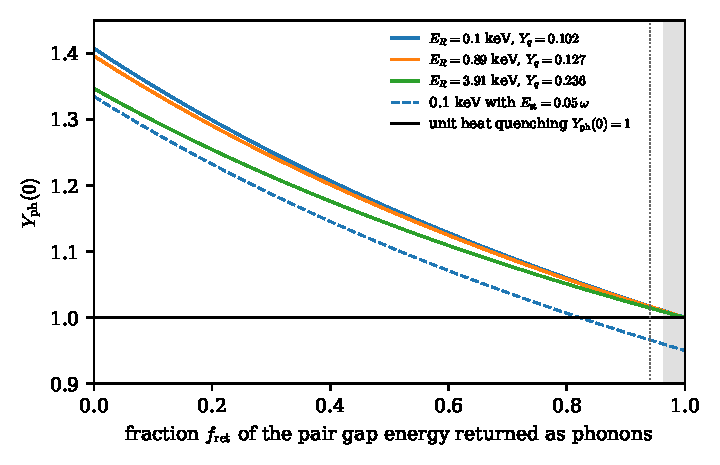
\includegraphics[width=\linewidth]{figures/ch19/limit19_5a.pdf}
\captionof{figure}{Heat quenching of silicon recoils from the release law \cref{eq:19.5-release} with $\delta_{\mathrm{coll}} = 0$, $\Delta E_{\mathrm{zp}} = 0$ and the same returned fraction $f_{\mathrm{ret}}$ for both recoils, against $f_{\mathrm{ret}}$. Solid: no stored energy, at the measured yields $Y_q$~\cite[Table~II]{albakry2023first} of 0.10, 0.89 and \SI{3.91}{keV}; $\Eg = \SI{1.17}{eV}$, $\varepsilon_{\mathrm{eh}} = \SI{3.75}{eV}$. Dashed: \SI{0.1}{keV} with a stored energy of $0.05\,\omega$. Horizontal line: the truncation. Gray: $f_{\mathrm{ret}} \ge 0.965$, where the \SI{0.1}{keV} curve lies within \SI{1}{\percent} of one. Dotted: $f_{\mathrm{ret}} = 0.941$, the asymptotic phonon share of the illustrative kinetics of \cref{fig:18-end}; there \SI{5}{\percent} of the pairs are trapped.}\label{fig:19-limit-heat}
\par}
\smallskip
When part of the gap energy is still held by pairs, excitons or traps at the end of the window, the electron recoil, with four to ten times more energy in pairs, loses more of its heat than the nuclear recoil, and the ratio rises above one, by up to \SI{41}{\percent} at \SI{100}{eV}; stored energy pulls it below.
\end{limitbox}

The truncation demands nearly complete release. Within \SI{1}{\percent} at \SI{100}{eV} requires $1 - f_{\mathrm{ret}} \le 0.035$, and the bound is nearly the same over the measured range, 0.036 at \SI{0.89}{keV} and 0.041 at \SI{3.91}{keV}, since the factor $(1 - Y_q)$ changes little while $Y_q$ stays small. A trapped fraction of a few percent, which no window removes, is already a percent-level violation, of opposite sign to the stored energy. The two effects can cancel in a single measurement, which is one reason a heat measurement alone determines neither.

\subsection{The phonon-yield ratio}\label{sec:19.5-yield}

With a bias the phonon signal has three parts: the primary phonons of the recoil, the Luke phonons of the drift and the recombination phonons that carriers emit at the contacts~\cite[Sect.~2]{agnese2018nuclear}. The recombination phonons carry gap energy returned within the window, and the balance law counts them with the primaries, in $E_{\mathrm{dep}} - E_{\mathrm{miss}}$; when drift collects the pairs within the window, $E_{\mathrm{miss}}$ holds the trapped carriers and their electrostatic energy, and the stored, escaped and zero-point energy. The sensors collect primary and Luke phonons with different efficiencies, because the two populations are born with different spectra and in different places. Let $\epsilon^{\mathrm{ER}}_{\mathrm{prim}}$ and $\epsilon^{\mathrm{NR}}_{\mathrm{prim}} = (1 - \delta_{\mathrm{coll}})\epsilon^{\mathrm{ER}}_{\mathrm{prim}}$ be the efficiencies for the primary phonons of the two recoils and $\epsilon_{\mathrm{Luke}}$ that for Luke phonons, and define the collection ratio
\begin{equation*}
  \mathfrak{r}_{\mathrm{coll}} \equiv \frac{\epsilon_{\mathrm{Luke}}}{\epsilon^{\mathrm{ER}}_{\mathrm{prim}}} ,
\end{equation*}
the efficiency for Luke phonons over that for the primary phonons of an electron recoil. Let the electron recoil be fully collected, so that its bias work is $g_{\mathrm{Luke}}\omega$ by \cref{eq:19.5-Wbias}, and define the ionized fraction $f_{\mathrm{ion}}$ of a nuclear recoil as its bias work over that of an electron recoil of the same energy, $f_{\mathrm{ion}} = N^{\mathrm{NR}}_{\mathrm{ind}}/N^{\mathrm{ER}}_{\mathrm{ind}}$. It equals the ionization yield $Y_q$ of \cref{eq:19.2-Yq} when both recoils are collected alike and is smaller if the carriers of the dense track are trapped more often. Per unit deposit the two signals are then
\begin{equation}
  \frac{S_{\mathrm{ER}}}{\epsilon^{\mathrm{ER}}_{\mathrm{prim}}\,\omega} = 1 - d_{\mathrm{ER}} + \mathfrak{r}_{\mathrm{coll}}\,g_{\mathrm{Luke}} , \qquad
  \frac{S_{\mathrm{NR}}}{\epsilon^{\mathrm{ER}}_{\mathrm{prim}}\,\omega} = (1 - \delta_{\mathrm{coll}})(1 - d_{\mathrm{NR}}) + \mathfrak{r}_{\mathrm{coll}}\,g_{\mathrm{Luke}}f_{\mathrm{ion}} .
  \label{eq:19.5-signal}
\end{equation}

The CDMS~II calibration turns these signals into energies in two steps~\cite[Eq.~(1), Sect.~2.1]{agnese2018nuclear}. The charge channel is calibrated with photon lines, so that an electron recoil of energy $\omega$ reads the electron-equivalent energy $E_Q = \omega$ and a nuclear recoil $E_Q = f_{\mathrm{ion}}\omega$. The phonon scale is set with bulk electron recoils, taken to have unit ionization yield, so that an electron recoil reads $E_\phi = \omega(1 + eV_{\mathrm{bias}}/\varepsilon_{\mathrm{cal}})$, and a nuclear recoil is assigned the energy $E_\phi - E_QeV_{\mathrm{bias}}/\varepsilon_{\mathrm{cal}}$. Note that $\varepsilon_{\mathrm{cal}}$ is the pair energy the reconstruction adopts, \SI{3.82}{eV} for silicon~\cite[Sect.~2]{agnese2018nuclear}, not the true $\varepsilon_{\mathrm{eh}}$. It enters both the scale and the subtraction, through the gain $g_{\mathrm{cal}} \equiv eV_{\mathrm{bias}}/\varepsilon_{\mathrm{cal}}$, while the Luke phonons follow the true pair number and $g_{\mathrm{Luke}}$. The phonon-yield ratio $Y_{\mathrm{ph}}$ is the reconstructed energy of the nuclear recoil over its true energy, which the CDMS~II analysis calls the phonon collection efficiency for nuclear recoils relative to electron recoils, and its deficit is the defect fraction $f_{\mathrm{DF}} \equiv 1 - Y_{\mathrm{ph}}$. From \cref{eq:19.5-signal},
\begin{equation}
  Y_{\mathrm{ph}} = (1 + g_{\mathrm{cal}})\,\frac{(1 - \delta_{\mathrm{coll}})(1 - d_{\mathrm{NR}}) + \mathfrak{r}_{\mathrm{coll}}g_{\mathrm{Luke}}f_{\mathrm{ion}}}{1 - d_{\mathrm{ER}} + \mathfrak{r}_{\mathrm{coll}}g_{\mathrm{Luke}}} - f_{\mathrm{ion}}g_{\mathrm{cal}} .
  \label{eq:19.5-identity}
\end{equation}
The absolute efficiency $\epsilon^{\mathrm{ER}}_{\mathrm{prim}}$ has cancelled. With no missing energy and $\mathfrak{r}_{\mathrm{coll}} = 1$ the ratio is $1 + (g_{\mathrm{cal}} - g_{\mathrm{Luke}})(1 - f_{\mathrm{ion}})/(1 + g_{\mathrm{Luke}})$, not one. For silicon at \SI{4}{V}, with $g_{\mathrm{Luke}} = 1.067$, $g_{\mathrm{cal}} = 1.047$ and $f_{\mathrm{ion}} = 0.324$, the pair energy alone produces a deficit of 0.0064, against the half-width 0.008 of the measured band. At zero bias \cref{eq:19.5-identity} is the heat quenching \cref{eq:19.5-heatq}, and multiplying out its denominator relates the two.
\begin{keyresult}[Calibration identity]
The phonon-yield ratio at bias $V_{\mathrm{bias}}$ and the heat quenching $Y_{\mathrm{ph}}(0)$ of the same recoils, with the same missing energies, are related by
\begin{equation}
  Y_{\mathrm{ph}} = \frac{(1 + g_{\mathrm{cal}})\,Y_{\mathrm{ph}}(0) + f_{\mathrm{ion}}(\mathfrak{r}'g_{\mathrm{Luke}} - g_{\mathrm{cal}})}{1 + \mathfrak{r}'g_{\mathrm{Luke}}} , \qquad
  \mathfrak{r}' = \frac{\mathfrak{r}_{\mathrm{coll}}}{1 - d_{\mathrm{ER}}} .
  \label{eq:19.5-calib}
\end{equation}
When $\mathfrak{r}'g_{\mathrm{Luke}} = g_{\mathrm{cal}}$, the calibrated ratio equals the heat quenching at every bias; for a reconstruction with the true pair energy this is $\mathfrak{r}' = 1$, Luke phonons collected like the available primary phonons of an electron recoil.
\end{keyresult}
\noindent The ratio $\mathfrak{r}'$ differs from $\mathfrak{r}_{\mathrm{coll}}$ by the missing energy of the calibrating electron recoils. Flashing, the exposure of the detectors to infrared light that neutralizes ionized traps before data taking~\cite[Sect.~2]{agnese2018nuclear}, keeps that energy small. Away from $\mathfrak{r}'g_{\mathrm{Luke}} = g_{\mathrm{cal}}$ the two ratios differ even when no energy is missing, since the Luke phonons, a larger share of the electron-recoil signal than of the nuclear one, then carry a different weight in the two.

The expansion of \cref{eq:19.5-identity} to first order in $\delta_{\mathrm{coll}}$ and the missing energies, derived in \cref{app:D.45}, displays the separate contributions:
\begin{equation}
\begin{split}
  1 - Y_{\mathrm{ph}} &= \frac{(\mathfrak{r}_{\mathrm{coll}}g_{\mathrm{Luke}} - g_{\mathrm{cal}})(1 - f_{\mathrm{ion}})}{1 + \mathfrak{r}_{\mathrm{coll}}g_{\mathrm{Luke}}} + \frac{1 + g_{\mathrm{cal}}}{1 + \mathfrak{r}_{\mathrm{coll}}g_{\mathrm{Luke}}}\bigl[\delta_{\mathrm{coll}} + d_{\mathrm{NR}} - C_{\mathrm{cal}}\,d_{\mathrm{ER}}\bigr] , \\
  C_{\mathrm{cal}} &= \frac{1 + \mathfrak{r}_{\mathrm{coll}}g_{\mathrm{Luke}}f_{\mathrm{ion}}}{1 + \mathfrak{r}_{\mathrm{coll}}g_{\mathrm{Luke}}} .
\end{split}
  \label{eq:19.5-first}
\end{equation}
The collection term is exact, and it is the whole answer when no energy is missing; it contains the pair-energy offset $g_{\mathrm{Luke}} - g_{\mathrm{cal}}$ together with $\mathfrak{r}_{\mathrm{coll}} - 1$. The calibration coefficient $C_{\mathrm{cal}}$ measures how much a deficit of the calibrating electron recoils matters. Such a deficit lowers the phonon scale and so raises every reconstructed nuclear-recoil energy. However, it acts through the primary part of the signal alone, and the nuclear recoil has less Luke signal to offset; as a result $C_{\mathrm{cal}} < 1$. For silicon at $\mathfrak{r}_{\mathrm{coll}} = 1$ and $f_{\mathrm{ion}} = 0.324$ it is 0.651 at \SI{4}{V} and 0.382 at \SI{40}{V}, and 0.62 to 0.74 at \SI{4}{V} for the ionized fractions of 10 to \SI{100}{keV}. Since \cref{eq:19.5-identity} is linear in $\delta_{\mathrm{coll}}$ and in $d_{\mathrm{NR}}$ separately, the first-order form errs through their product and through $d_{\mathrm{ER}}$: by at most $3.0\times10^{-3}$ when each of the three lies between 0 and 0.05.

Write the missing energy of the nuclear recoil as $d_{\mathrm{NR}} = e_{\mathrm{st}} + x_{\mathrm{NR}}$, with $e_{\mathrm{st}} \equiv E_{\mathrm{st}}/\omega$ the stored fraction, and $x_{\mathrm{ER}} = d_{\mathrm{ER}}$ for the electron recoil, so that $x$ collects trapped, escaped and zero-point energy. Electron recoils store almost no energy. The largest energy an electron of kinetic energy $E$ gives a silicon nucleus is $2E(E + 2m_e)/M_\kappa$, which reaches the lowest threshold, \SI{12.5}{eV}, at $E = \SI{0.14}{MeV}$; whatever the calibrating electrons do store counts in $x_{\mathrm{ER}}$. \Cref{app:D.45} shows that \cref{eq:19.5-identity} implies, without approximation,
\begin{multline}
  (1 - Y_{\mathrm{ph}} - e_{\mathrm{st}})(1 - x_{\mathrm{ER}} + \mathfrak{r}_{\mathrm{coll}}g_{\mathrm{Luke}}) = (\mathfrak{r}_{\mathrm{coll}}g_{\mathrm{Luke}} - g_{\mathrm{cal}})(1 - e_{\mathrm{st}} - f_{\mathrm{ion}}) \\
  + (1 + g_{\mathrm{cal}})\bigl[\delta_{\mathrm{coll}}(1 - e_{\mathrm{st}}) + (1 - \delta_{\mathrm{coll}})x_{\mathrm{NR}}\bigr] - (1 - e_{\mathrm{st}} + f_{\mathrm{ion}}g_{\mathrm{cal}})\,x_{\mathrm{ER}} .
  \label{eq:19.5-bound}
\end{multline}
The factor $1 - x_{\mathrm{ER}} + \mathfrak{r}_{\mathrm{coll}}g_{\mathrm{Luke}}$ is positive. The right side is non-negative, and the stored fraction is therefore at most the defect fraction, $E_{\mathrm{st}}/\omega \le 1 - Y_{\mathrm{ph}}$, under five conditions on collection, missing energy and the reconstruction:
\begin{description}
\item[(a)] $\delta_{\mathrm{coll}} \ge 0$: the primary phonons of nuclear recoils are collected no better than those of electron recoils.
\item[(b)] $\mathfrak{r}_{\mathrm{coll}} \ge 1$: Luke phonons are collected no worse than the primaries of electron recoils.
\item[(c)] $(1 + g_{\mathrm{cal}})(1 - \delta_{\mathrm{coll}})x_{\mathrm{NR}} \ge (1 - e_{\mathrm{st}} + f_{\mathrm{ion}}g_{\mathrm{cal}})x_{\mathrm{ER}}$: at small deficits, the other missing energy of the nuclear recoil is at least $(1 + f_{\mathrm{ion}}g_{\mathrm{cal}})/(1 + g_{\mathrm{cal}})$ times that of the electron recoil. It holds, for instance, when the electron recoils lose nothing to traps after flashing and the zero-point change of the defects is not negative.
\item[(d)] $e_{\mathrm{st}} \le 1 - f_{\mathrm{ion}}$, met with a wide margin at stored fractions of a few percent.
\item[(e)] $\varepsilon_{\mathrm{eh}} \le \varepsilon_{\mathrm{cal}}$: the true pair energy is no larger than the one the reconstruction adopts, so that with (b) $\mathfrak{r}_{\mathrm{coll}}g_{\mathrm{Luke}} \ge g_{\mathrm{cal}}$. For germanium it refers to the pair energy of the germanium analysis, whose offset is not evaluated here.
\end{description}
The measured silicon pair energy, \SI{3.75}{eV} (\cref{sec:18.4}), meets (e) against the \SI{3.82}{eV} of the CDMS~II reconstruction; were $\varepsilon_{\mathrm{eh}}$ above $\varepsilon_{\mathrm{cal}}$, the first term would turn negative and the bound would loosen. At \SI{95}{\percent} confidence the silicon datum has $Y_{\mathrm{ph}} \ge 0.945$, so $E_{\mathrm{st}}/\omega \le 0.055$ under (a)--(e). With the book's $\varepsilon_{\mathrm{eh}}$ the pair-energy term is known, and under (a)--(d) the bound is tighter, 0.049, attained at $\mathfrak{r}_{\mathrm{coll}} = 1$ with no other deficit, since the first term of \cref{eq:19.5-bound} grows with $\mathfrak{r}_{\mathrm{coll}}$. A negative zero-point change violates (c) and widens the bound by $|\Delta E_{\mathrm{zp}}|/\omega$. With \SI{0.1}{eV} per displacement and the displacement count of \cref{lim:19.4a}, that is $8\times10^{-4}$ at \SI{10}{keV}, and the bound for either sign of $\Delta E_{\mathrm{zp}}$ is 0.056. \Cref{sec:19.4} collects the silicon and germanium bounds in \cref{tab:19-bounds}.

Condition (b) is the weak one. Luke phonons are emitted with energies of a few meV at most, softer than the primary phonons. In the films that collect phonons, the part of their spectrum below the pair-breaking energy $2\Delta_{\mathrm{BCS}}$ of aluminum, \SI{0.36}{meV} (\cref{sec:1.5}), is lost energy, as is the part absorbed at bare surfaces. The sign of $\mathfrak{r}_{\mathrm{coll}} - 1$ is therefore not fixed by the balance law. The mean-field transport estimate of \cref{sec:20.5-sign} puts the collection ratio between 0.81 and 1.02, and between 0.82 and 1.01 at the mean Luke energy of silicon electrons at \SI{1}{V/cm}, for one or two films of any thickness down to \SI{60}{nm} with energy conserved; values up to 1.5 arise only for a selective sink that the estimate does not identify in a detector. For a stated detector \cref{app:E.25} specifies the calculation. On the branch $\mathfrak{r}_{\mathrm{coll}} < 1$, with $\delta_{\mathrm{coll}} = x_{\mathrm{NR}} = x_{\mathrm{ER}} = 0$, \cref{eq:19.5-identity} solved for the stored energy is
\begin{equation}
  \frac{E_{\mathrm{st}}}{\omega} = 1 - Y_{\mathrm{ph}} + \frac{(g_{\mathrm{cal}} - \mathfrak{r}_{\mathrm{coll}}g_{\mathrm{Luke}})(Y_{\mathrm{ph}} - f_{\mathrm{ion}})}{1 + g_{\mathrm{cal}}} ,
  \label{eq:19.5-widen}
\end{equation}
so the inferred stored fraction grows linearly as $\mathfrak{r}_{\mathrm{coll}}$ falls. For the central silicon datum it is 0.042 at $\mathfrak{r}_{\mathrm{coll}} = 1$, 0.058 at 0.95 and 0.075 at 0.9, and the \SI{95}{\percent} bound reaches 0.081 at 0.9. The bound is void if nothing bounds $\mathfrak{r}_{\mathrm{coll}}$ from below.

\begin{limitbox}[Stored energy from the phonon-yield ratio][lim:19.5b]
The defect fraction read as stored energy~\cite[Eq.~(4)]{agnese2018energy}, \cite[Eq.~(1)]{agnese2018nuclear}: $E_{\mathrm{st}}/\omega = f_{\mathrm{DF}} = 1 - Y_{\mathrm{ph}}$, the case $\mathfrak{r}_{\mathrm{coll}} = 1$, $\delta_{\mathrm{coll}} = x_{\mathrm{NR}} = x_{\mathrm{ER}} = 0$, $\varepsilon_{\mathrm{cal}} = \varepsilon_{\mathrm{eh}}$ of \cref{eq:19.5-identity}, with $Y_{\mathrm{ph}} = 0.952^{+0.009}_{-0.007}$ (\SI{95}{\percent} C.L.) measured in silicon at \SI{4}{V}~\cite[Sect.~4]{agnese2018nuclear}.
\par\smallskip
{\centering
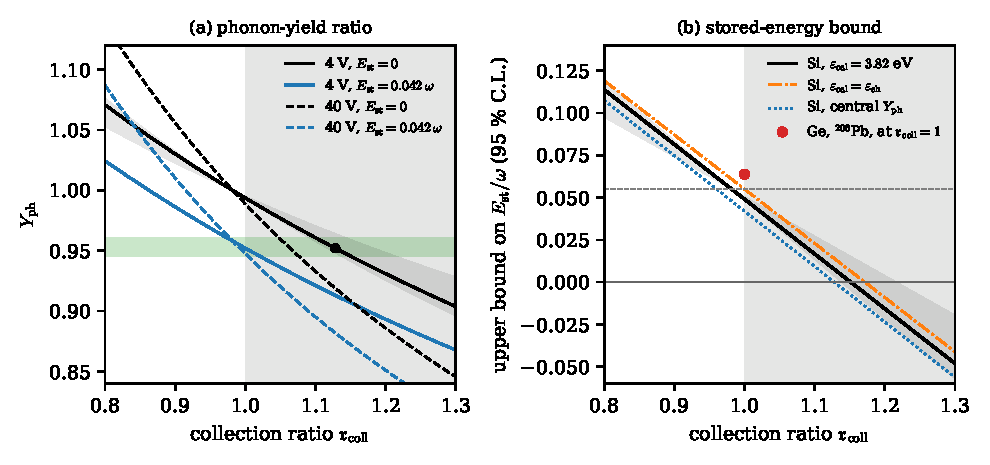
\includegraphics[width=\linewidth]{figures/ch19/limit19_5b.pdf}
\captionof{figure}{Silicon recoils against the collection ratio, from the exact identity \cref{eq:19.5-identity} with $\delta_{\mathrm{coll}} = d_{\mathrm{ER}} = 0$, $g_{\mathrm{Luke}} = 1.067$ ($\varepsilon_{\mathrm{eh}} = \SI{3.75}{eV}$) and $g_{\mathrm{cal}} = 1.047$ ($\varepsilon_{\mathrm{cal}} = \SI{3.82}{eV}$) at \SI{4}{V}, ten times both at \SI{40}{V}, and $f_{\mathrm{ion}} = 0.324$, the yield parameterization of the measurement at the \SI{20}{keV} resonance that dominates the calibration~\cite[Eq.~(4)]{agnese2018nuclear}. (a) Phonon-yield ratio. Black: no stored energy; blue: stored fraction 0.042; solid at \SI{4}{V}, dashed at \SI{40}{V}. Dark band: $f_{\mathrm{ion}}$ from 0.269 to 0.497, the same parameterization at 10 and \SI{100}{keV}. Green: the measured $0.952^{+0.009}_{-0.007}$. Dot: $\mathfrak{r}_{\mathrm{coll}} = 1.128$, where collection alone reproduces it. (b) Upper bound on $E_{\mathrm{st}}/\omega$ at \SI{95}{\percent} confidence, \cref{eq:19.5-widen} at $Y_{\mathrm{ph}} = 0.945$, with the band of (a); dotted: the central $Y_{\mathrm{ph}}$; dash-dotted: a reconstruction with the true pair energy; dashed line: the literature reading 0.055. Red point: germanium at $\mathfrak{r}_{\mathrm{coll}} = 1$. Gray: $\mathfrak{r}_{\mathrm{coll}} \ge 1$, where under (a)--(e) the bound does not exceed $f_{\mathrm{DF}}$.}\label{fig:19-limit-yield}
\par}
\smallskip
Below $\mathfrak{r}_{\mathrm{coll}} = 1$ the bound exceeds $f_{\mathrm{DF}}$, 0.081 at $\mathfrak{r}_{\mathrm{coll}} = 0.9$ for silicon; above $\mathfrak{r}_{\mathrm{coll}} = 1.128$ the central silicon datum needs no stored energy, and the datum alone cannot tell the two readings apart (\cref{we:19-degeneracy}).
\end{limitbox}

The collection offset has a part that the balance law fixes. The recombination phonons at the contacts carry the gap energy of the collected pairs, the fraction $\Eg/\varepsilon_{\mathrm{eh}}$ of an electron-recoil deposit and $f_{\mathrm{ion}}\Eg/\varepsilon_{\mathrm{eh}}$ of a nuclear one, and they are born at the surfaces next to the sensors, with their own spectrum. Let $\rho_g$ be their collection efficiency over that of the hard primary phonons, $\epsilon_{\mathrm{hard}}$. A recoil whose gap fraction is $\chi_g\Eg/\varepsilon_{\mathrm{eh}}$, with $\chi_g = 1$ for the electron and $\chi_g = f_{\mathrm{ion}}$ for the nuclear recoil, then has the primary efficiency $\epsilon_{\mathrm{hard}}[1 + (\rho_g - 1)\chi_g\Eg/\varepsilon_{\mathrm{eh}}]$. The gap part of the offset is
\begin{equation}
  \delta^{\mathrm{gap}}_{\mathrm{coll}} = \frac{(1 - f_{\mathrm{ion}})(\Eg/\varepsilon_{\mathrm{eh}})(\rho_g - 1)}{1 + (\Eg/\varepsilon_{\mathrm{eh}})(\rho_g - 1)} .
  \label{eq:19.5-dgap}
\end{equation}
In silicon at $f_{\mathrm{ion}} = 0.324$, $\rho_g - 1 = 0.21$ gives $\delta^{\mathrm{gap}}_{\mathrm{coll}} = 0.042$, which alone accounts for the deficit of the datum beyond the pair-energy offset, and a change of 0.02 in $\rho_g$ moves it by 0.0037. Contacts sit on the same faces as the sensors, so a difference of this size is possible; its value needs a transport calculation for the detector (\cref{app:E.25}). The rest of the offset comes from the primary spectra, which differ little once down-conversion has erased their origin (\cref{sec:20.2}); from the depth profiles of the calibration sources, since neutrons and gammas do not interact at the same depths; and from escape at the surfaces, which differs between the two.

\subsection{Two-bias inversion of the silicon datum}\label{sec:19.5-inversion}

The CDMS~II silicon detectors were biased at \SI{4}{V} across \SI{1}{cm}, and their neutron calibration gives $Y_{\mathrm{ph}} = 0.952^{+0.009}_{-0.007}$ over 10 to \SI{100}{keV}~\cite[Sects.~2, 4]{agnese2018nuclear}. \Cref{we:19-degeneracy} reads this one number in the two limiting ways.

\begin{workedexample}{The degeneracy of the silicon datum between stored energy and collection}\label{we:19-degeneracy}
The Luke gain is $g_{\mathrm{Luke}} = \SI{4}{V}/\SI{3.75}{V} = 1.067$, and the reconstruction uses $g_{\mathrm{cal}} = \SI{4}{V}/\SI{3.82}{V} = 1.047$. The calibration rests on the spectral feature that an elastic resonance of silicon puts at recoil energies near \SI{20}{keV}~\cite[Sect.~3.2]{agnese2018nuclear}. There the ionization of nuclear recoils is collected in full and follows the yield parameterization of the same analysis~\cite[Eq.~(4), Sect.~4]{agnese2018nuclear}, $y_C = [1/(a_CE_R) + 1/y_L]^{-1}$ with $a_C = \SI{0.247}{keV^{-1}}$ and $y_L$ Lindhard's yield \cref{eq:16.6-lindhard}. It gives $f_{\mathrm{ion}} = 0.324$; Lindhard's yield alone, which overestimates the low-energy data that analysis cites, gives 0.346; the same analysis notes that its fit improves if $y_C$ is about \SI{5}{\percent} low at 10 to \SI{20}{keV}, which the Lindhard variant covers. We set $\delta_{\mathrm{coll}} = x_{\mathrm{NR}} = x_{\mathrm{ER}} = 0$.

\emph{Stored energy alone.} With $\mathfrak{r}_{\mathrm{coll}} = 1$, \cref{eq:19.5-widen} is
\begin{equation*}
  e_{\mathrm{st}} = 1 - Y_{\mathrm{ph}} + \frac{(g_{\mathrm{cal}} - g_{\mathrm{Luke}})(Y_{\mathrm{ph}} - f_{\mathrm{ion}})}{1 + g_{\mathrm{cal}}} = 0.048 - 0.006 = 0.042 ,
\end{equation*}
and 0.049 at the lower edge of the band. The pair-energy offset takes an eighth of the deficit; read with $\varepsilon_{\mathrm{cal}} = \varepsilon_{\mathrm{eh}}$, the datum would give 0.048 and 0.055. Lindhard's $f_{\mathrm{ion}}$ changes the stored fraction by $2\times10^{-4}$.

\emph{Collection alone.} With $E_{\mathrm{st}} = 0$ the collection term of \cref{eq:19.5-first} remains, $1 - Y_{\mathrm{ph}} = (\mathfrak{r}_{\mathrm{coll}}g_{\mathrm{Luke}} - g_{\mathrm{cal}})(1 - f_{\mathrm{ion}})/(1 + \mathfrak{r}_{\mathrm{coll}}g_{\mathrm{Luke}})$, and solving for the collection ratio,
\begin{equation*}
  \mathfrak{r}_{\mathrm{coll}} = \frac{(1 - Y_{\mathrm{ph}}) + g_{\mathrm{cal}}(1 - f_{\mathrm{ion}})}{g_{\mathrm{Luke}}(Y_{\mathrm{ph}} - f_{\mathrm{ion}})} = \frac{0.048 + 0.708}{0.670} = 1.128 .
\end{equation*}
Luke phonons collected \SI{13}{\percent} better than the primaries reproduce the datum with no stored energy. The band of the datum maps onto $1.099 \le \mathfrak{r}_{\mathrm{coll}} \le 1.152$, and Lindhard's $f_{\mathrm{ion}}$ gives 1.134. The mean-field transport estimate of \cref{sec:20.5-sign} puts the collection ratio between 0.81 and 1.02 with energy conserved, and only a selective sink that the estimate does not identify in a detector reaches higher values. Collection alone, $\mathfrak{r}_{\mathrm{coll}} = 1.128$, is therefore not reached by the transport estimate, but it is not excluded until computed kernels test real detectors (\cref{app:E.25}); the two-bias measurement of \cref{sec:19.5-inversion} decides.

\emph{Mixtures.} Every point of the line \cref{eq:19.5-widen} reproduces the datum: half of the stored-energy reading, $e_{\mathrm{st}} = 0.021$, needs $\mathfrak{r}_{\mathrm{coll}} = 1.064$. A gap offset \cref{eq:19.5-dgap} with $\rho_g - 1 = 0.21$ reproduces it with neither.

\emph{Energy dependence.} At fixed $\mathfrak{r}_{\mathrm{coll}} = 1.128$ the collection term scales with $1 - f_{\mathrm{ion}}$, and $f_{\mathrm{ion}}$ grows with the recoil energy: the parameterization gives 0.269 at \SI{10}{keV} and 0.497 at \SI{100}{keV}, hence $Y_{\mathrm{ph}} = 0.948$ and 0.964, the second just above the upper edge 0.961 of the band. The same analysis finds, however, that the ionization collected at \SI{4}{V/cm} falls to about \SI{75}{\percent} of the parameterized yield at \SI{100}{keV}~\cite[Sect.~4]{agnese2018nuclear}; with $f_{\mathrm{ion}} = 0.75 \times 0.497 = 0.373$ the prediction is 0.956, inside the band. A stored fraction independent of energy predicts 0.951 to 0.954 over the range. At the present precision the energy dependence does not separate the readings.
\end{workedexample}

A second bias separates the collection ratio from the rest. Multiply \cref{eq:19.5-identity} by its denominator and divide by $1 - d_{\mathrm{ER}}$: at the bias $V_i$, with gains $g_{\mathrm{Luke},i}$ and $g_{\mathrm{cal},i}$,
\begin{equation}
  (1 + g_{\mathrm{cal},i})\,Y_{\mathrm{ph}}(0) - g_{\mathrm{Luke},i}\,(Y_i - f_{\mathrm{ion}})\,\mathfrak{r}' = Y_i + f_{\mathrm{ion}}g_{\mathrm{cal},i} ,
  \label{eq:19.5-linear}
\end{equation}
with $Y_i$ the phonon-yield ratio measured at that bias and $Y_{\mathrm{ph}}(0)$ and $\mathfrak{r}'$ those of \cref{eq:19.5-calib}. The relation is exact and linear in the two unknowns. Two biases give two equations whose determinant is $(Y - f_{\mathrm{ion}})(g_{\mathrm{Luke},1} - g_{\mathrm{Luke},2})$ when the two measured ratios are equal and does not vanish in general, so the pair $(Y_{\mathrm{ph}}(0), \mathfrak{r}')$ follows by solving a $2\times2$ system (\cref{app:D.45}). For silicon at 4 and \SI{40}{V}, collection alone ($\mathfrak{r}_{\mathrm{coll}} = 1.128$, no stored energy) predicts $Y_{\mathrm{ph}} = 0.919$ at \SI{40}{V}, stored energy alone 0.947, since the pair-energy offset grows with the bias, and the half-and-half mixture 0.932. Solving \cref{eq:19.5-linear} with these values returns the inputs. The difference between the readings, 0.028, is about 3.6 times the half-width of the present band, and an uncertainty of 0.005 on the \SI{40}{V} ratio moves the inverted $\mathfrak{r}'$ by 0.020 to 0.026. At still higher bias the Luke phonons dominate both signals and $Y_{\mathrm{ph}}$ tends to $f_{\mathrm{ion}} + [Y_{\mathrm{ph}}(0) - f_{\mathrm{ion}}]\varepsilon_{\mathrm{eh}}/(\varepsilon_{\mathrm{cal}}\mathfrak{r}')$, which is 0.912 for collection alone.

The inversion holds under hypotheses that are each a missing input. The collection ratio must not change between the two biases, yet the spectrum of Luke phonons depends on the field; the residual is of order $(\dd\mathfrak{r}_{\mathrm{coll}}/\dd V_{\mathrm{bias}})\,\Delta V_{\mathrm{bias}}$, which the transport calculation of \cref{app:E.25} provides. The ionized fraction must be measured at both biases with the charge channel, since trapping depends on the field. The offset and the missing energies must also be the same at both biases, which requires both to collect every pair within the window; a zero-bias run does not qualify as the second point, because the gap energy of uncollected pairs then enters through \cref{eq:19.5-release}. Finally, the reconstruction must use the same $\varepsilon_{\mathrm{cal}}$ at both biases and the true $\varepsilon_{\mathrm{eh}}$ must be known, since \cref{eq:19.5-linear} carries the two gains separately. A third bias overdetermines \cref{eq:19.5-linear} and tests the first three hypotheses.

What the inversion cannot do is split $Y_{\mathrm{ph}}(0) = (1 - \delta_{\mathrm{coll}})(1 - d_{\mathrm{NR}})/(1 - d_{\mathrm{ER}})$ into collection offset and stored energy, since both enter it in the same way. Three further measurements or calculations split it. Transport calculations of the efficiencies of each phonon population in the detector that took the data fix the gap and spectral parts of $\delta_{\mathrm{coll}}$ (\cref{app:E.25}). Neutron and gamma sources with matched depth profiles remove its position part. And two read windows, short and long, separate stored energy released within the window from energy that stays frozen, since the release term of $d_{\mathrm{NR}}$ is the one that grows with $t_{\mathrm{win}}$.
